%%%%%%%%%%%%%%%%%%%%%%%%%%%%%%%%%%%%%%%%%%%%%%%%%%%%%%%%%%%%%%%%%%%%%%%%
% Preamble
%%%%%%%%%%%%%%%%%%%%%%%%%%%%%%%%%%%%%%%%%%%%%%%%%%%%%%%%%%%%%%%%%%%%%%%%
\documentclass[12pt]{article}
%
% Packages and other includes
% Pagination
\usepackage[letterpaper, margin=1in]{geometry}
%
% Graphics, floats, tables
\usepackage{graphicx, color, float, array}
\graphicspath{{image/}}
%
% Fonts
\usepackage[T1]{fontenc} % best for Western European languages
\usepackage{lmodern} % Latin Modern instead of CM
\usepackage{textcomp} % required to get special symbols
%
% Math
\usepackage{amsmath, amssymb}
\usepackage{enumerate}
\usepackage{braket}
% 
% Hyperlinks
\usepackage[colorlinks,linkcolor={red},citecolor={blue},
urlcolor={blue}]{hyperref} 
%
% Definitions and settings
% Paragraph indent and spacing
\setlength{\parskip}{0.4\baselineskip}
\setlength{\parindent}{0in}
%
% Math mode version of "r" column type (requires array package)
\newcolumntype{R}{>{$}r<{$}}
% Title, authors, date
\title{\textbf{Light Energy, Quantum Numbers, and Periodic Trends}}
\date{Nov 6, 2023}

\begin{document}

\maketitle 

\textbf{Light Energy and Bohr Model}

1) Describe the Bohr Model. What is the model's limitation(s)?

\vspace{1.5in}

2) Calculate the energy (E) and wavelength ($\lambda$) of a photon of light with a frequency ($\nu$)
of $6.165 \times 10^{14}$ Hz. Compute the energy for a mole of photons.

\vspace{1.5in}

3) For the hydrogen emissions and absorption, describe what regions of the electromagnetic
radiation spectrum do the Lyman series, Balmer series, and Paschen series reside.

\begin{center}
  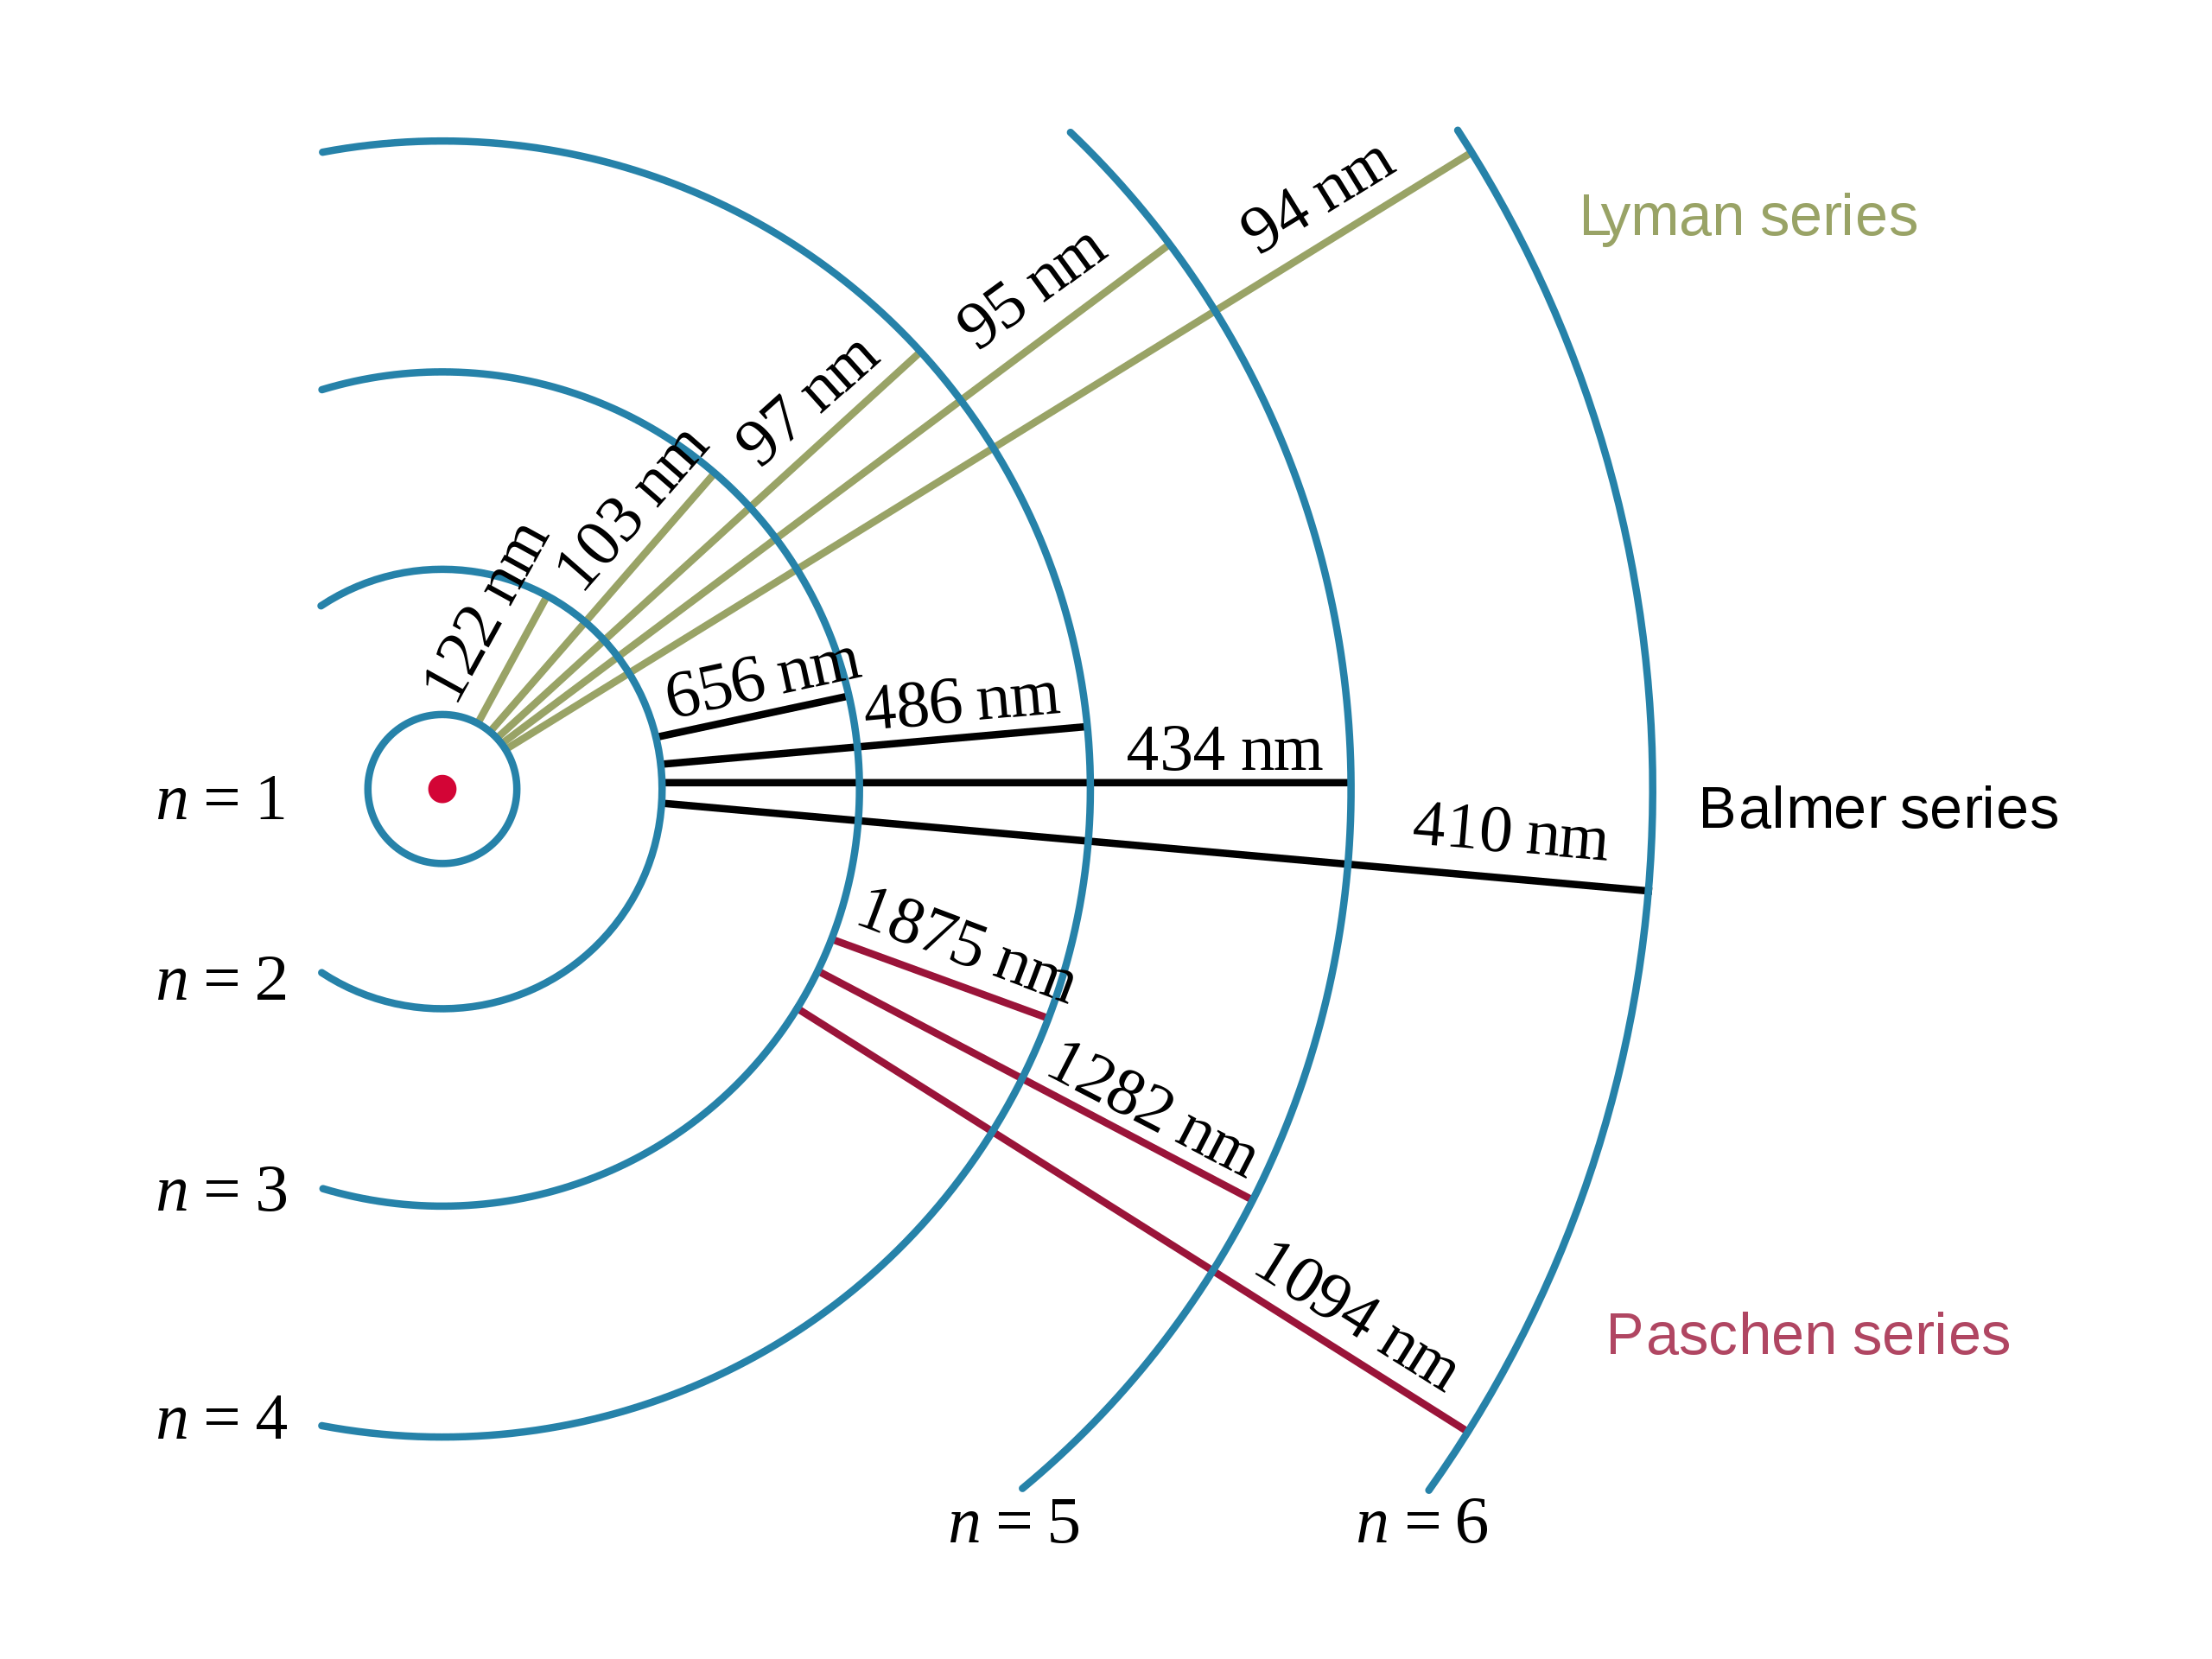
\includegraphics[scale=0.12]{h_transition}
\end{center}

4) Another way to write the Rydberg equation is the following:
\begin{equation}
  \Delta E = 2.18 \times 10^{-18}\text{ J}\Big(\frac{1}{n_i} - \frac{1}{n_f}\Big)
\end{equation}
Obtain the equation from the formula shown in class.
\begin{equation}
  \frac{1}{\lambda} = 1.097 \times 10^{-2}\text{ nm}\Big(\frac{1}{n_i} - \frac{1}{n_f}\Big)
\end{equation}

\vspace{1.75in}

5) An electron from a hydrogen atom emits a wavelength of 433 nm falling to $n = 2$. Determine
what initial energy level $n$ did the electron fall from.

\vspace{1.75in}

6) Light with a frequency of is $2.1 \times 10^{15}$ Hz incident on a metal whose work function is
$7.21 \times 10^{-19}$. Determine the velocity of emitted electrons. (Hint: Kinetic energy is
$\frac{1}{2}mv^2$ where $m$ is the mass of electron $9.109 \times 10^{31}$ kg and $v$ is the
velocity.)

\vspace{1.75in}

7) For the classical and quantum pictures of light energy, describe the differences and
similarities for emission and absorption. Draw a energy level diagram to illustrate this point.

\vspace{2in}

\textbf{Quantum Numbers and Electron Configuration}

8) Define the Heisenberg Uncertainty principle.

\vspace{1.5in}

9) For energy level $n=4$, what values of $l$, $m_l$, and $m_s$ are allowed?

\vspace{2in}

10) Write the electron configurations both the long and shorthanded ways.

a) Ag

b) Pb

c) Hg

d) Ra

e) Yb

\vspace{1in}

11) Draw the orbital diagram of Na and Cl satisfying the Aufbau principle and Hund's rule to
fill the orbitals.

\vspace{1.5in}

\textbf{Periodic Trends}

12) Describe why the atomic radius of a neutral atom shrinks going across the periodic table. Why does the
atomic radius increase going down the column?

\vspace{1.5in}

13) Describe the trend for electronegativity. Determine the following bonds 
are ionic or covalent based on the difference between electronegativity. Use the ptable website.

a) H-Cl

b) Na-Cl

c) O-H

d) O-F

\end{document}
